\section{\texttt{Folding.hs}}

The tree of configurations is folded into a graph using the 
well-known technique of ``tying the knot''
(\url{http://www.haskell.org/haskellwiki/Tying_the_Knot}).
We traverse the tree top-down, accumulating the encountered configurations.
If the current configuration coincides with a previous one modulo renaming,
then a loop is formed and we do not go inside the corresponding subtree.

\begin{lstlisting}[name=folding]
foldTree :: Tree Conf -> Graph Conf
foldTree t = fixTree (tieKnot []) t

tieKnot :: [Node Conf] -> Node Conf -> Tree Conf 
	-> Graph Conf
tieKnot ns n t@(Node e _) =
	case [(k, r) | k <- n:ns, isCall e, 
			Just r <- [renaming (nodeLabel k) e]] of
		[] -> fixTree (tieKnot (n:ns)) t
		(k, r):_ -> Node e (Fold k r)

fixTree :: (Node t -> Tree t -> Graph t) -> Tree t 
	-> Graph t
fixTree f (Node e (Transient c)) = t where
	t = Node e $ Transient $ f t c
fixTree f (Node e (Decompose cs)) = t where
	t = Node e $ Decompose [f t c | c <- cs]
fixTree f (Node e (Variants cs)) = t where
	t = Node e $ Variants [(p, f t c) | (p, c) <- cs]
fixTree f (Node e Stop) = (Node e Stop)
\end{lstlisting}

The following example is shown in the main article, subsection ``Folding''.
\begin{lstlisting}[style=demo]
-- demo15
ghci> foldTree $ buildTree (driveMachine prog1) 
	{{even(sqr(x))}}
...

\end{lstlisting}

We repeat the graph drawing here, marking coinciding (up to renaming) nodes
with the same color.

\begin{landscape}
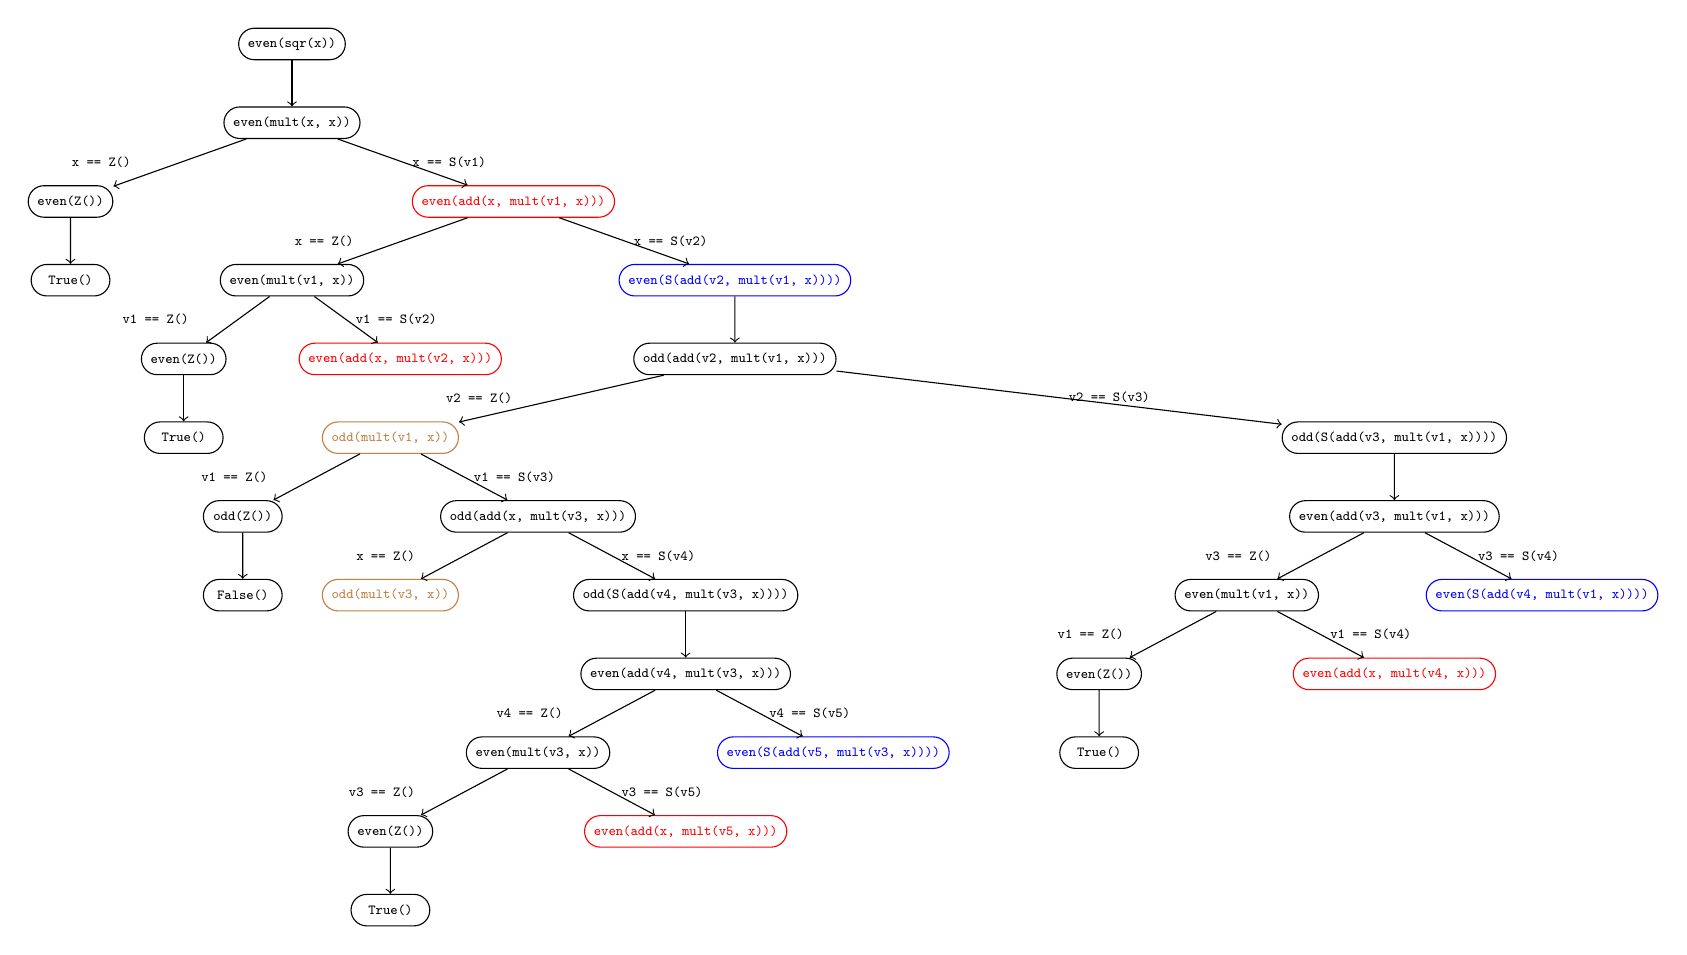
\begin{tikzpicture}[scale=1.25,
level distance=8mm,
level/.style={sibling distance=20mm},
conf/.style={
	rectangle,minimum width=10mm,minimum height=4mm,rounded corners=2mm,
	draw=black,
	font=\ttfamily\tiny},
label/.style={font=\ttfamily\tiny}
]
\tikzstyle{level 2}=[sibling distance=45mm]
\tikzstyle{level 3}=[sibling distance=45mm]
\tikzstyle{level 4}=[sibling distance=22mm]
\tikzstyle{level 5}=[sibling distance=70mm]
\tikzstyle{level 6}=[sibling distance=30mm]
\tikzstyle{level 7}=[sibling distance=30mm]
\tikzstyle{level 8}=[sibling distance=30mm]
\tikzstyle{level 9}=[sibling distance=30mm]
\tikzstyle{level 10}=[sibling distance=30mm]
\node[conf]{even(sqr(x))}
child[->]{node[conf]{even(mult(x, x))}
child[->]{node[conf]{even(Z())}
child[->]{node[conf]{True()}}
edge from parent node[left,label,xshift=-5mm]{x == Z()}}
child[->]{node[conf,red]{even(add(x, mult(v1, x)))}
child[->]{node[conf]{even(mult(v1, x))}
child[->]{node[conf]{even(Z())}
child[->]{node[conf]{True()}}
edge from parent node[left,label,xshift=-5mm]{v1 == Z()}}
child[->]{node[conf,red]{even(add(x, mult(v2, x)))}
edge from parent node[right,label]{v1 == S(v2)}}
edge from parent node[left,label,xshift=-5mm]{x == Z()}}
child[->]{node[conf,blue]{even(S(add(v2, mult(v1, x))))}
child[->]{node[conf]{odd(add(v2, mult(v1, x)))}
child[->]{node[conf,brown]{odd(mult(v1, x))}
child[->]{node[conf]{odd(Z())}
child[->]{node[conf]{False()}}
edge from parent node[left,label,xshift=-5mm]{v1 == Z()}}
child[->]{node[conf]{odd(add(x, mult(v3, x)))}
child[->]{node[conf,brown]{odd(mult(v3, x))}
edge from parent node[left,label,xshift=-5mm]{x == Z()}}
child[->]{node[conf]{odd(S(add(v4, mult(v3, x))))}
child[->]{node[conf]{even(add(v4, mult(v3, x)))}
child[->]{node[conf]{even(mult(v3, x))}
child[->]{node[conf]{even(Z())}
child[->]{node[conf]{True()}}
edge from parent node[left,label,xshift=-5mm]{v3 == Z()}}
child[->]{node[conf,red]{even(add(x, mult(v5, x)))}
edge from parent node[right,label]{v3 == S(v5)}}
edge from parent node[left,label,xshift=-5mm]{v4 == Z()}}
child[->]{node[conf,blue]{even(S(add(v5, mult(v3, x))))}
edge from parent node[right,label]{v4 == S(v5)}}}
edge from parent node[right,label]{x == S(v4)}}
edge from parent node[right,label]{v1 == S(v3)}}
edge from parent node[left,label,xshift=-5mm]{v2 == Z()}}
child[->]{node[conf,xshift=40mm]{odd(S(add(v3, mult(v1, x))))}
child[->]{node[conf]{even(add(v3, mult(v1, x)))}
child[->]{node[conf]{even(mult(v1, x))}
child[->]{node[conf]{even(Z())}
child[->]{node[conf]{True()}}
edge from parent node[left,label,xshift=-5mm]{v1 == Z()}}
child[->]{node[conf,red]{even(add(x, mult(v4, x)))}
edge from parent node[right,label]{v1 == S(v4)}}
edge from parent node[left,label,xshift=-5mm]{v3 == Z()}}
child[->]{node[conf,blue]{even(S(add(v4, mult(v1, x))))}
edge from parent node[right,label]{v3 == S(v4)}}}
edge from parent node[right,label]{v2 == S(v3)}}}
edge from parent node[right,label]{x == S(v2)}}
edge from parent node[right,label]{x == S(v1)}}}
;

\end{tikzpicture}
\end{landscape}
